% Chapter 2
\chapter{Descrizione generale} % Main chapter title
%----------------------------------------------------------------------------------------

% Define some commands to keep the formatting separated from the content 
% \newcommand{\keyword}[1]{\textbf{#1}}

%----------------------------------------------------------------------------------------
\section{Prospettiva del prodotto}
Il prodotto software sarà un'applicazione basata su un'architettura a tre livelli, composta da due macro-componenti indipendenti: una parte di \textit{back-end} e una di \textit{front-end}. 

\textbf{Back-end} \\
Avrà la responsabilità della gestione centralizzata dello stato del sistema, garantendo che tutte le informazioni e i dati persistenti siano conservati e aggiornati unicamente su di esso.

\textbf{Front-end} \\
Costituirà l'interfaccia utente che si appoggierà ai servizi REST esposti dal back-end.

\section{Funzioni del prodotto}
In questo paragrafo sono stati elencati i requisiti funzionali utente, dedotti dalle funzionalità descritte nel primo capitolo, e descritti mediante i diagrammi di caso d'uso.
Il paragrafo è suddiviso in due parti:

\begin{quote}
Nella \textit{prima parte} verrà fornito un elenco dei requisiti funzionali dedotti dalle specifiche del committente. 
Tali requisiti sono descritti con un linguaggio chiaro, comprensibile anche a parsone senza un'approfonddita conoscenza tecnica.     
\end{quote}

\begin{quote}
Nella \textit{seconda parte} verranno presentati i diagrammi di caso d'uso, i quali saranno associati a uno o più requisiti.
\end{quote}

\subsection{Requisiti funzionali utente}
\begin{quote}
\begin{enumerate}[label=\textit{RF\arabic*}]
  \item \textbf{Il sistema deve offrire un meccanismo di autenticazione.}
    
  \item \textbf{Il sistema deve poter permettere a ogni account \textit{Amministratore} di creare ulteriori utenti, sia normali che di tipo amministratore, specificando le loro credenziali di accesso. }
  
  \item \textbf{Gli utenti possono segnalare issue, con la possibilità di specificare un titolo, una descrizione, una priorità, una immagine e il tipo.}
  
  \item \textbf{Il sistema deve permettere la visualizzazione di tutte le issue segnalate, con la possibilità di filtrare e ordinare i risultati.}
  
  \item \textbf{Il sistema deve permettere, solo a un \textit{Amministratore}, di assegnare bug e notificare un membro del team.}
  
  \item \textbf{Il sistema deve consentire a un \textit{utente normale} di ricevere notifiche riguardanti i bug.}

  \item \textbf{Ogni \textit{utente normale} può visualizzare i propri bug assegnati.}

  \item \textbf{Il sistema deve fornire una funzione di ricerca per trovare issue.}

  \item \textbf{Il sistema dovrebbe suggerire  automaticamente a chi assegnare un bug.}
  
\end{enumerate} 
\end{quote}

\subsection{Diagrammi di caso d'uso} 

Qui di seguito vengono illustrati i diagrammi di caso d'uso che modellano i requisiti sopra citati.

\begin{figure}[!ht] 
\begin{center}
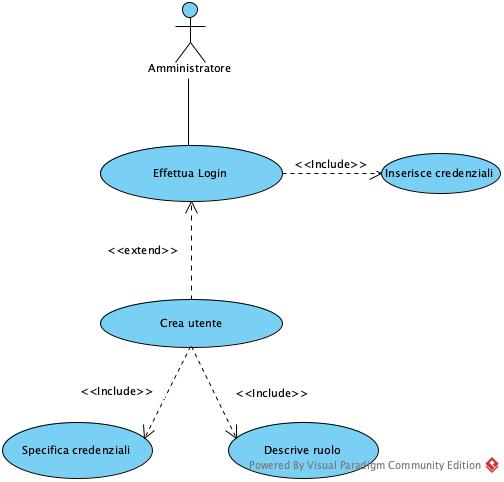
\includegraphics[width=10cm]{Chapters/Punto1.jpg}
\end{center}
\caption{Modellazione requisiti \textit{RF1}, \textit{RF2}}
\label{fig:f1} 
\end{figure}

\begin{figure}[!ht] 
\begin{center}
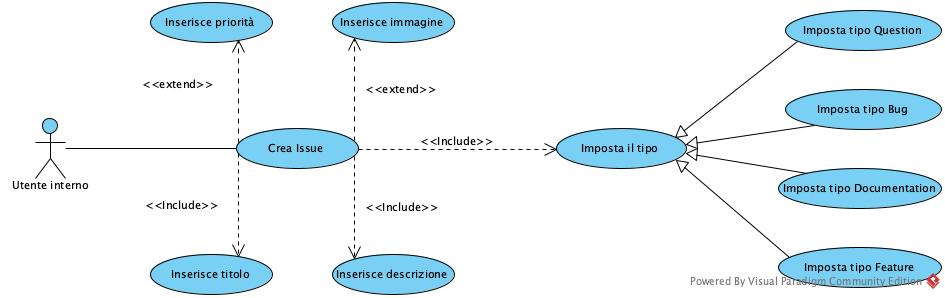
\includegraphics[width=15cm]{Chapters/Punto2.jpg}
\end{center}
\caption{Modellazione requisito \textit{RF3}}
\label{fig:f2} 
\end{figure}

\begin{figure}[!ht] 
\begin{center}
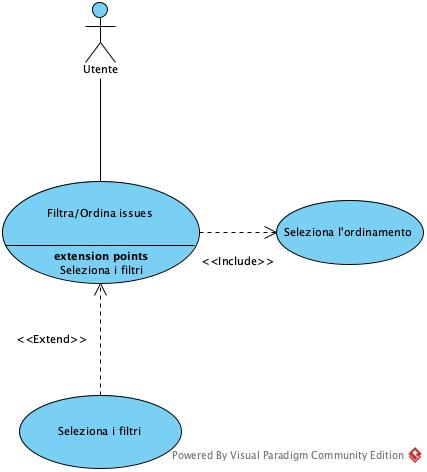
\includegraphics[width=10cm]{Chapters/Punto3.jpg}
\end{center}
\caption{Modellazione requisito \textit{RF4}}
\label{fig:f3} 
\end{figure}

\begin{figure}[!ht] 
\begin{center}
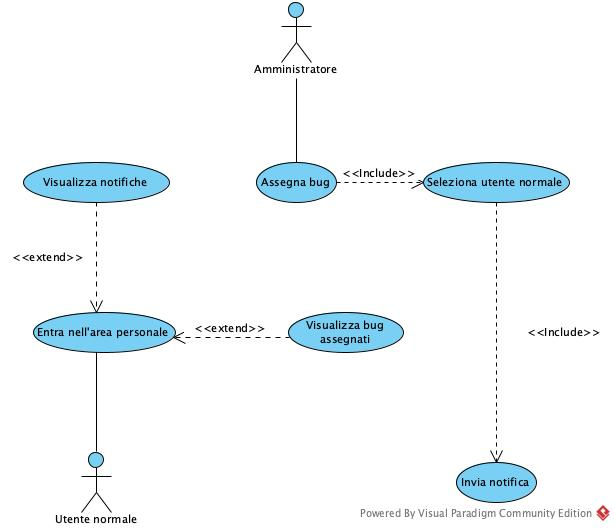
\includegraphics[width=12cm]{Chapters/Punto4.jpg}
\end{center}
\caption{Modellazione requisiti \textit{RF5}, \textit{RF6}, \textit{RF7}}
\label{fig:f4} 
\end{figure}

\begin{figure}[!ht] 
\begin{center}
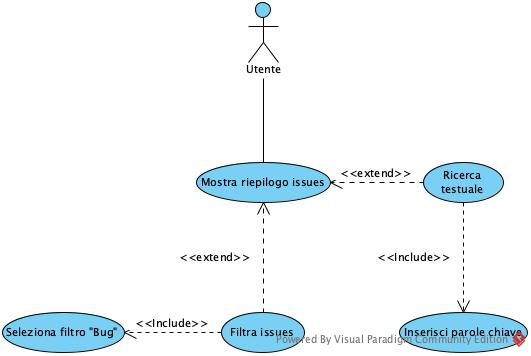
\includegraphics[width=12cm]{Chapters/Punto11.jpg}
\end{center}
\caption{Modellazione requisiti \textit{RF4}, \textit{RF8}}
\label{fig:f5} 
\end{figure}

\begin{figure}[!ht] 
\begin{center}
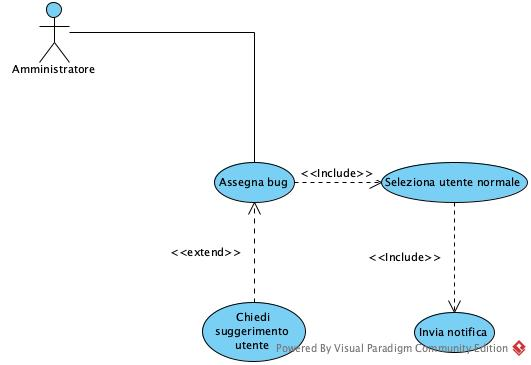
\includegraphics[width=15cm]{Chapters/Punto14.jpg} 
\end{center}
\caption{Modellazione requisiti \textit{RF5},\textit{RF9}}
\label{fig:f6} 
\end{figure}

% \begin{figure}
%     \centering
%     
\includegraphics[width=.6\textwidth]{Dedication/dedication.pdf}
%     \caption{An example dedication page.}
%     \label{fig:chap2:dedication_sample}
% \end{figure}


\clearpage

\section{Caratteristiche utente}
L'utilizzo di questo prodotto software da parte degli utenti richiede 
che questi ultimi abbiano una buona conoscenza del dominio applicativo 
in cui il software opera. Per tale motivo, gli utenti del sistema sono 
stati divisi in due categorie in funzione del ruolo ricoperto.

\begin{enumerate}
  \item \textit{utente normale}
  \item \textit{utente mministratore}
\end{enumerate}

Gli \textit{utenti amministratori} sono coloro che utilizzano tutte le funzionalità messe a disposizione dal sistema. \\ 
\indent Gli \textit{utenti normali}, invece, utilizzano un sottoinsieme limitato delle funzionalità, pur possedendo una conoscenza approfondita del dominio applicativo. 
È il caso, in particolare, dei membri di un team di sviluppo. Questi devono essere in grado di riconoscere e saper descrivere chiaramente i loro problemi (bug, suggerimento di nuove funzionalità, ecc.). \\
\indent Per qualsiasi tipologia di utente, una scarsa conoscenza del dominio applicativo può portare all'incapacità di riconoscere e  descrivere correttamente tali problemi, con conseguente perdita di tempo e potenziali fraintendimenti.
Nello specifico, le definizioni e i ruoli dei singoli attori del sistema sono:

\textbf{Amministratore}\\
Si riferisce a un utente che ha accesso completo al sistema, senza limitazione alcuna. Tra le operazioni che può effettuare figurano la gestione degli utenti e la gestione dei bug (come ad esempio, l'assegnazione di un bug a un membro del team).

\textbf{Utente normale}\\
Chiamato anche utente \textit{regolare}, si riferisce a un utente senza privilegi speciali. Il suo ruolo è quello di segnalare problemi, proporre miglioramenti o fare richieste funzionali. \\
\indent Tali account vengono assegnati normalmente ai membri di un team di sviluppo, i quali possono anche visualizzare i bug assegnati in un'apposita sezione.

\section{Presupposti e dipendenze}

\subsection{Dipendenze tecnologiche}
\begin{itemize}
  \item \textit{Containerizzazione del back-end}: Il committente desidera che una componente del software, ovvero la parte di \textit{back-end}, sia distribuita utilizzando tecnologie di containerizzazione come \textit{Docker}.

  \begin{itemize}
  \item \textit{Dipendenze}: Si assume che le macchine server supportino l'esecuzione di \textit{container} \textit{Docker}, includendo un demone \textit{Docker} installato correttamente e configurato.    
\end{itemize}
\end{itemize}

\subsection{Dipendenze sull'ambiente dell'utente}
\begin{itemize}
  \item \textit{Connettività di rete}: L'architettura di sistema prevede 
  che il \textit{front-end} comunichi con il \textit{back-end} anche 
  quando questo risiede in una rete esterna.
  \begin{itemize}
  \item \textit{Dipendenze}: Qualora le parti si trovino in due reti separate, 
  si assume che gli utenti finali dispongano 
  di una connessione Internet stabile e affidabile per poter utilizzare 
  l'applicazione senza interruzioni. La qualità dell'esperienza utente 
  dipenderà direttamente dalle prestazioni della rete.
\end{itemize}
\end{itemize}
